\documentclass{amsart}
% \documentclass{article}
\usepackage{ifxetex}
\ifxetex
\usepackage{fontspec}
\usepackage{xunicode}
\usepackage{xltxtra}
\usepackage{xecyr}
\setmainfont[Mapping=tex-text,Ligatures=TeX]{CMU Serif}
\usepackage{polyglossia}
\setdefaultlanguage{english, russian}
\else
\usepackage[utf8]{inputenc}
\usepackage[T2A]{fontenc}
% \usepackage{concrete}
\fi

\usepackage{fullpage}
\usepackage{eufrak}
\usepackage{listings}
\usepackage{todonotes}
\usepackage{color}
\usepackage{xcolor}
\usepackage{enumitem}
% \usepackage{ntheorem}
\usepackage{amsthm,amsmath,amsfonts,amssymb}

%formatting
\usepackage[left=2.5cm,right=2.5cm,top=2cm,bottom=2cm,bindingoffset=0cm]{geometry}
\renewcommand{\baselinestretch}{1.2}
\sloppy

%tikz graphics
\usepackage{tikz}
\usetikzlibrary {positioning}
\usetikzlibrary{automata}
\usetikzlibrary{arrows,shapes}
\tikzstyle{vertex}=[circle,fill=black,minimum size=3pt,inner sep=0pt]
\tikzstyle{edge} = [draw,thick,-]

\newtheorem*{theorem}{Theorem}
\newtheorem*{lemma}{Lemma}
\newtheorem*{fact}{Fact}
\newtheorem*{rem}{Remark}
\newtheorem*{cor}{Corollary}

\newenvironment{task}[2] {
	\noindent\fbox{\bf {#1} {#2}}
}{
}

\newcommand{\mytitle}[2] {
	\begin{center}
		\bf {#1} {#2}
	\end{center}
}

\let\origenumerate\enumerate
\let\origendenumerate\endenumerate
\renewenvironment{enumerate}{\origenumerate[topsep = 0pt, noitemsep]}{\origendenumerate}

\usepackage[backend=bibtex]{biblatex}
\addbibresource{map.bib}

\begin{document}
	\mytitle{}{Reduction map}
	
\begin{figure}[!htp]
	
	\begin{center}  
		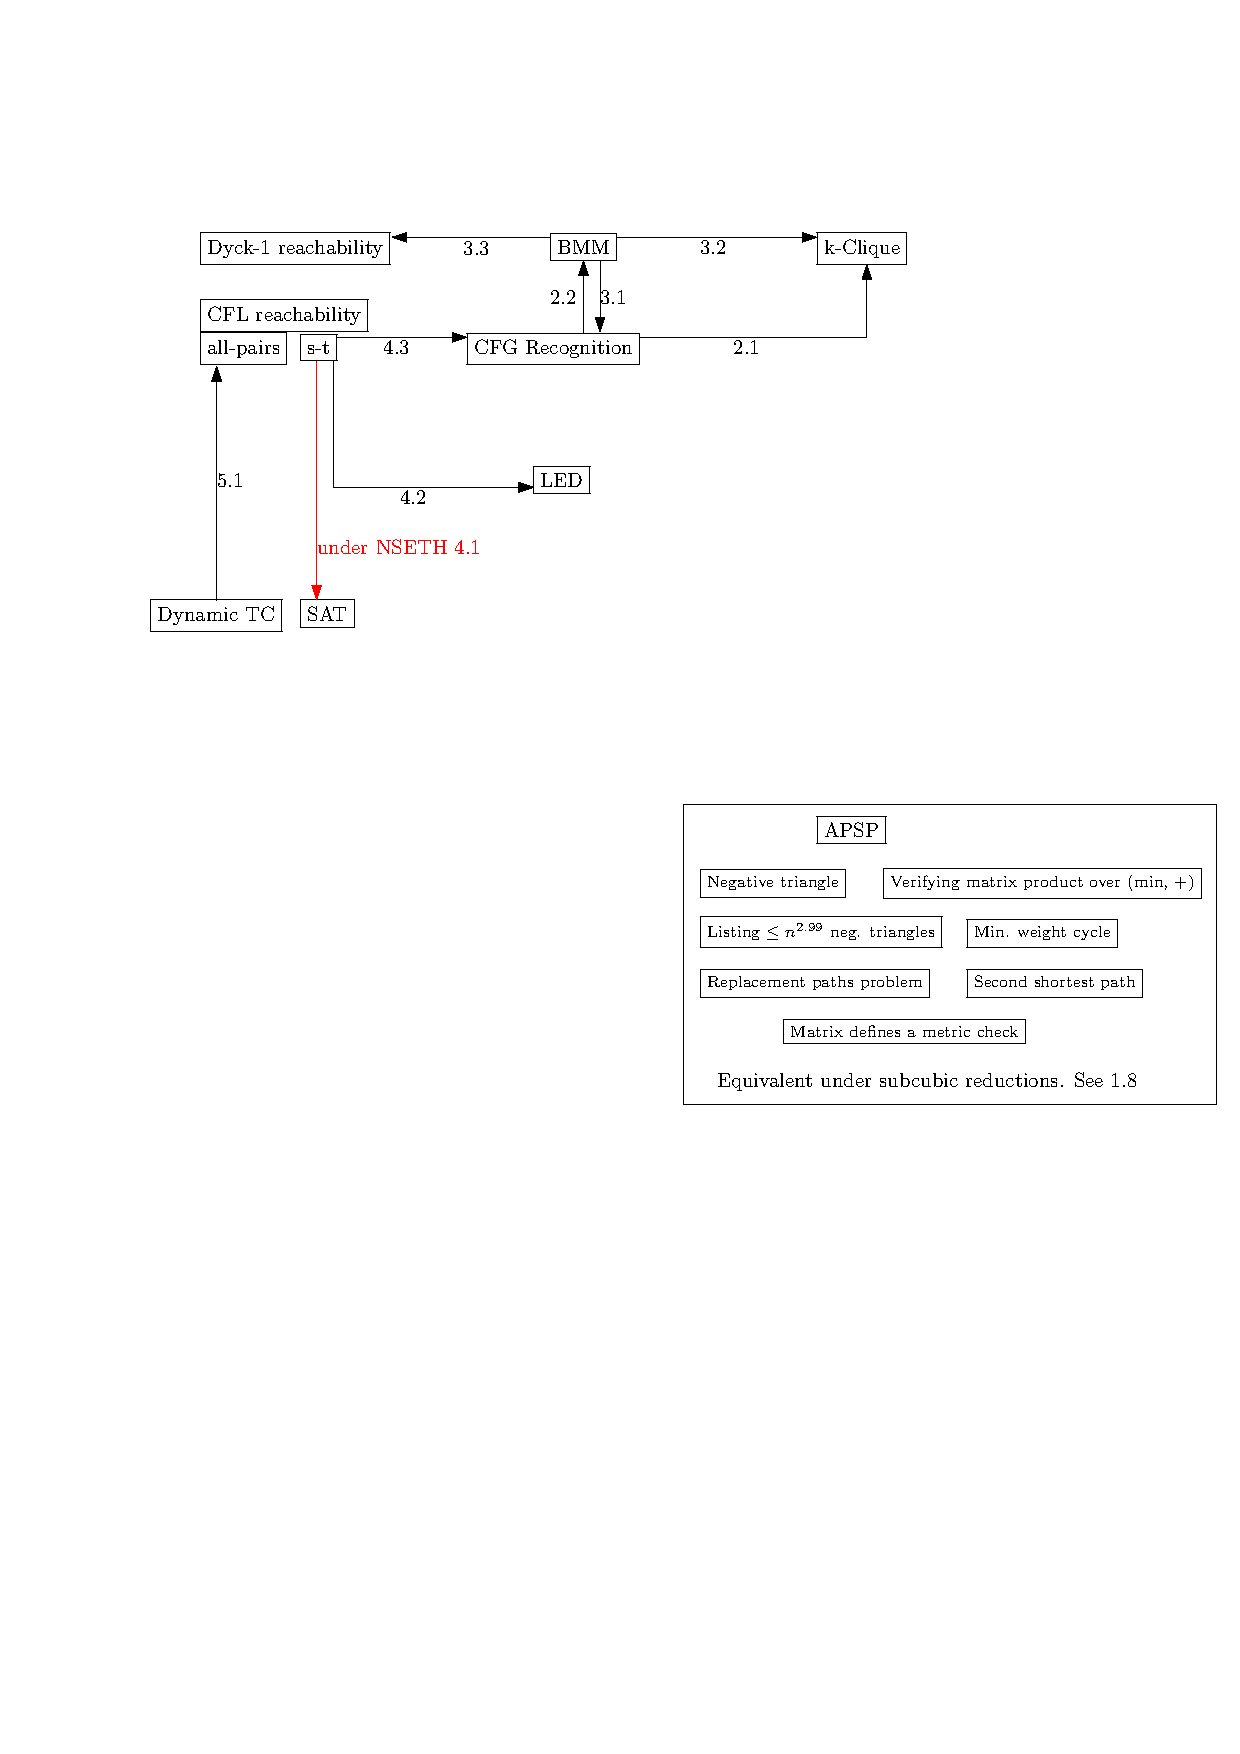
\includegraphics[scale = 0.8]{map.pdf}
	\end{center}
		
\end{figure}
	
	$A \rightarrow B \Longleftrightarrow$ B has reduction to A
	
	{\color{red} $\longrightarrow$} -- no reduction
	
	{\color{blue} hypothesis}
	
	\section{Problem definitions}
	
	\subsection{CFG recognition:}
	
	given a CFG $\mathcal{G}$ and a string $w \in \Sigma^*$ determine if $w$ can be obtained from $G$ (i.e. whether $w \in \mathcal{L}(\mathcal{G})$)
	
	Best upper bound~\cite{valiant1975general}: $\mathcal{O}(n^{\omega} \cdot |\mathcal{G}|^2)$
	
	Best combinatorial algorithms: $\mathcal{O}(n^3 / \log^3 n)$
	
	\textbf{CFG parsing problem:} if $w \in \mathcal{L}(\mathcal{G})$, output a
	possible derivation sequence.
	
	CFG recognition is as hard as CFG parsing up to logarithmic factors~\cite{10.5555/646233.682379}.
	
	\subsection{CFL reachability:}
	
	given a CFG $\mathcal{L}$ and a labelled graph $G$
	
	\subsection{k-Clique:}
	
	decide whether a given undirected unweighted graph on n nodes and $\mathcal{O}(n^2)$ edges contains a clique on $k$ nodes.
	
	It is a parameterized version of the NP-hard Max-Clique problem.
	
	Let $0 \leq F \leq \omega$ and $0 \leq C \leq 3$ be the smallest numbers such that $3k$-Clique can be solved combinatorially in $O(n^{Ck})$ time and in $O(n^{Fk})$ time by any algorithm, for any (large enough) constant $k \geq 1$. A conjecture in graph algorithms and parameterized complexity is that $C = 3$ and $F = \omega$.
	
	\subsection{SAT}
	
	\subsubsection{$k$-SAT:}
	
	Given a $k$-CNF formula $\phi$ on $n$ variables. Is there an assignment to the variables that satisfies $\phi$?
	
	\subsubsection{ETH (Exponential time hypothesis):}
	
	There is no algorithm that solves $k$-SAT in time $2^{o(n)}$ for any $k$.
	
	\subsubsection{SETH (Strong exponential time hypothesis):} 
	
	There is no $\epsilon > 0$ such that k-SAT can be solved in time $2^{(1-\epsilon)n}$ for any $k$.
	
	\subsubsection{NSETH (Nondeterministic strong exponential time hypothesis):} 
	
	There is no $\epsilon > 0$ such that $k$-SAT can be solved in time $2^{(1-\epsilon)n}$ co-nondeterministically for any $k$.
	
	\subsection{BMM}
	
	Given two $n \times n$ matrices $A, B$ over $\{0, 1\}$, Boolean Matrix Multiplication (BMM) is $(AB)[i,j] = \vee_{k = 1}^n (A(i,k) \wedge B(k, j))$. 
	
	Note that BMM can be computed using an algorithm for integer matrix multiplication in $\mathcal{O}(n^{\omega})$ time. Still, no combinatorial $\mathcal{O}(n^{3 - \epsilon})$ algorithm is known.
	
	\subsubsection{BMM conjecture~\cite{10.1109/FOCS.2014.53}}
	In the Word RAM model with words of $\mathcal{O}(\log n)$ bits, any combinatorial algorithm requires $n^{3 - o(1)}$ time in expectation to compute the boolean product of two $n \times n$ matrices.
	
	\subsection{LED}
	
	Given a string $w \in \Sigma^*$ and a context-free grammar $\mathcal{G}$ defined over the same alphabet, how many minimum number of repairs (insertions, deletions and substitutions) are required to map $w$ into a valid member of $\mathcal{G}$?
	
	\subsection{3SUM}
	Determine whether a set $S \subset \{-n^3, \ldots, n^3\}$ of $|S|= n$ integers contains three distinct elements $a, b, c \in S$ with $a + b = c$.
	
	\subsubsection{3SUM conjecture}
	In the Word RAM model with words of $\mathcal{O}(\log n)$ bits, any algorithm requires $n^{2 - o(1)}$ time in expectation to solve 3SUM problem.
	
	\subsection{Triangle detection}
	
	\subsubsection{Triangle conjecture}
	There is a constant $\delta > 0$, such that in the Word RAM model with words of $\mathcal{O}(\log n)$ bits, any algorithm requires $m^{1 + \delta - o(1)}$ time in expectation to detect whether an $m$ edge graph contains a triangle.
	
	\subsection{APSP (all pairs shortest paths) and others~\cite{10.1145/3186893}:}
	\label{apsp_equiv}
	
	\begin{itemize}
		\item The all-pairs shortest paths problem on weighted digraphs (APSP).
		\item Detecting if a weighted graph has a triangle of negative total edge weight.
		\item Listing up to $n^{2.99}$ negative triangles in an edge-weighted graph.
		\item Finding a minimum weight cycle in a graph of non-negative edge weights.
		\item The replacement paths problem on weighted digraphs.
		\item Finding the second shortest simple path between two nodes in a weighted digraph.
		\item Checking whether a given matrix defines a metric.
		\item Verifying the correctness of a matrix product over the $(min, +)$-semiring (distance product).
	\end{itemize}
	
	\subsubsection{APSP conjecture}
	There is a constant $c$, such that in the Word RAM model with words of $\mathcal{O}(\log n)$ bits, any algorithm requires $n^{3 - o(1)}$ time in expectation to compute the distances between every pair of vertices in an $n$ node graph with edge weights in $\{1, \ldots, n^c\}$.
	
	\subsubsection{Negative Triangles Over Structures.}
	
	The negative triangle problem over $\mathcal{R}$ is defined on a weighted tripartite graph with parts $I, J, K$. Edge weights between $I$ and $J$ are from $\mathbb{Z}$, and all other edge weights are from
	$\mathcal{R}$. The problem is to detect if there are $i \in I, j \in J, k \in K$ so that $(w(i, k) \bigodot w(k, j)) + w(i, j) < 0$. Note that if one negates all weights of edges between $I$ and $J$, the condition becomes $(w(i, k) \bigodot(k, j)) < w(i, j)$.
	
	In the special case when $\bigodot = +$ and $\mathcal{R} \subseteq \mathbb{Z} \cup \{ -- \infty, \infty\}$, the tripartiteness requirement is unnecessary, and the negative triangle problem is defined on an arbitrary graph with edge weights from $\mathbb{Z} \cup \{ -- \infty, \infty\}$. This
	holds for the negative triangle problem over both the $(min, +)$ and Boolean semirings.
	
	Note that detecting and finding one negative triangle in a graph problems reduce one to another:
	
	\begin{lemma}[Folklore]
		Let $T(n)$ be a function so that $\frac{T(n)}{n}$ is nondecreasing. If there is a $T(n)$ time
		algorithm for negative triangle detection over $\mathcal{R}$ on a graph $G = (I \cup J \cup K, E)$, then there is an $\mathcal{O}(T(n))$ algorithm which returns a negative triangle over $\mathcal{R}$ in $G$ if one exists.
	\end{lemma}

	\subsection{OV}
	
	The input to the Orthogonal Vectors (OV) problem is two sets $X, Y$, each containing $n$ vectors in $\{0, 1\}^D$, for some dimension $D = \omega(\log n)$. The task is to determine if there exists a pair $(x, y) \in (X, Y)$ that is orthogonal, i.e., for each $j \in D$, we have $x[j] \cdot y[j] = 0$. 
	
	The respective hypothesis states that the problem cannot be solved in time $\mathcal{O}(n^{2 - \epsilon})$, for any fixed $\epsilon > 0$.
	
	\section{To CFG recongnition}
	
	\subsection{From k-Clique problem~\cite{abboud2018if}:\\}
	\label{cfg_to_clique}
	
	Summary: $T(n) \Rightarrow \mathcal{O}(T(n^{k/3+1}) \; (|G|=\mathcal{O}(1))$
	
	\subsection{From BMM~\cite{10.1145/505241.505242}:\\}
	\label{cfg_to_bmm}
	
	Summary: $\mathcal{O}(|G| \cdot n^{3 - \epsilon}) \Rightarrow \mathcal{O}(m^{3 - \epsilon/3}) \; (|G|=\Omega(n^6)!)$, combinatorial reduction
	
	\section{To BMM}
	
	\subsection{From CFG recognition~\cite{valiant1975general}:\\}
	\label{bmm_to_cfg}
	
	Summary: $\mathcal{O}(n^{\omega}) \Rightarrow \mathcal{O}(n^{\omega})$
	
	\subsection{From k-Clique~\cite{nevsetvril1985complexity},~\cite{10.1016/j.tcs.2004.05.009}:\\}
	\label{bmm_to_clique}
	
	Summary: $\mathcal{O}(n^{\omega}) \Rightarrow \mathcal{O}(n^{i + \omega \cdot l}), k = 3 \cdot l + i, i = 0, 1, 2$ 
	
	or $\mathcal{O}(n^{\omega(\lfloor k / 3 \rfloor, \lfloor (k - 1) / 3 \rfloor, \lfloor k / 3 \rfloor)}$, where $\mathcal{O}(n^{\omega(r, s, t)})$ denotes the running time of the multiplication of an $n^r \times n^s$ matrix by an $n^s \times n^t$ matrix.
	
	Note that detecting arbitrary $k$-vertex (induced or not) subgraph in $n$-vertex graph is of the same complexity as detecting k-clique~\cite{nevsetvril1985complexity}.
	
	\subsection{From Dyck-1 reachability~\cite{bradford2017efficient},~\cite{10.1145/3434315}:\\}
	\label{bmm_to_dyck1}
	
	Summary: $\mathcal{O}(n^{\omega}) \Rightarrow \mathcal{O}(n^{\omega} \cdot \log^2 n)$, combinatorial reduction~\cite{10.1145/3434315}
	
	Idea: find bell-shaped paths in $\mathcal{O}(\log n n^{\omega})$ by getting $\mathcal{O}(\log n)$ transitive closures; combine Dyck-1 path from bell-shaped paths: in each of $\mathcal{O}(\log n)$ iterations we remove bell-shaped paths of height at most $2^i, i = 1, \ldots, \log n$.
	
	or $\mathcal{O}(n^{\omega}) \Rightarrow \mathcal{O}(n^{\omega} \cdot \log^3 n)$ in~\cite{bradford2017efficient} via algebraic matrix encoding of flat Dyck1-Reachability to $\mathcal{O}(\log n)$ AGMY matrix multiplications.
	
	\section{To CFL reachability}
	
	\subsection{To s-t reachability from SAT~\cite{chistikov2021subcubic}:\\}
	\label{dmchistikov}
	
	Summary: subcubic certificates for CFL reachability (positive and negative), no reductions under NSETH from SAT (SETH) to CFL reachability.
	
	Proof is based on the following lemma, where by instance $(G, \lambda, s, t)$ of CFL reachability problem $G$ is a graph, $\lambda$ is edge-labelling function, $s, t$ are vertices between which we search a path labelled with word from the language. 
	
	\begin{lemma}
		Let $(G,\lambda,s,t)$ be an instance of the CFL reachability problem. There is a linear-time reduction (in the bit-size of the input) to an instance $(G',\lambda',s',t')$ of the Dyck-2 reachability problem.
	\end{lemma}
	
	\subsection{To s-t reachability from LED}
	\label{cfl_to_led}
	
	Naive reduction: build a path graph labelled with letters of $w$, add loops marked with every symbol of $\Sigma$ on every vertex, add edges marked with every symbol of $\Sigma$ and $\epsilon$ between pairs of adjacent vertices. Make original edges of zero weight, edges with $\Sigma$ and $\epsilon$ symbols of positive weight (you can choose different weight-cost for different operations). Find path between end vertices marked with word formed from grammar with minimum weight.
	
	\subsection{To s-t reachability from CFG recognition~\cite{10.1145/3158118}:\\}
	\label{stcfl_to_cfg}
	
	Summary: $\mathcal{O}(n^{3 - \epsilon}) \Rightarrow \mathcal{O}(n^{3 - \epsilon})$, combinatorial
	
	\begin{lemma}
		If there exists a combinatorial algorithm that solves the pair Dyck reachability problem in time $T(n)$, where $n$ is the number of nodes of the input graph, then there exists a combinatorial
		algorithm that solves the CFL parsing problem in time $\mathcal{O}(n +T(n))$.
	\end{lemma}
	
	In combination with reduction to BMM we have:
	
	\begin{theorem}[BMM-hardness: Conditional cubic lower bound] 
		For any fixed $\epsilon > 0$, if there is a combinatorial algorithm that solves the pair Dyck reachability problem in $\mathcal{O}(n^{3 - \epsilon})$ time, then
		there is a combinatorial algorithm that solves Boolean Matrix Multiplication in $\mathcal{O}(n^{3 - \epsilon})$ time.
	\end{theorem}
	
	\section{To Dynamic TC}
	
	\subsection{From all-pairs CFL reachability~\cite{inbook}:\\}
	\label{dtc_to_cfl}
	
	Summary: $\mathcal{O}(n^{3 - \epsilon}) \Rightarrow \mathcal{O}(n^{3 - \epsilon})$
	
	\section{To Dyck-1 Reachability}
	
	\subsection{From OV (inspired by~\cite{10.1145/3434315}):\\}
	\label{dyck1_to_ov}
	
	{\color{red} Not working idea!}

	Summary: $\mathcal{O}(n^{2 - \epsilon}) \Rightarrow \mathcal{O}(n^{2 - \epsilon})$
	
	\begin{figure}[!htp]
		
		\begin{center}  
			\includegraphics[scale = 0.6]{ov_to_dyck1.pdf}
		\end{center}
	\label{fig:ov_to_dyck}
	
	\caption{Part of the reduction graph $G$ for vectors $x_1, y_1 \in \{0, 1\}^D, D = 2$. \\ Blue edges exist if the corresponding coordinates equal 0. }
		
	\end{figure}
	
	\emph{Intuition.} Without loss of generality suppose $D$ is even. Consider the first two vectors of the given sets: $x_1 \in X, y_1 \in Y$. Let us build part of the Dyck-1 graph $G$ that will check orthogonality of $x_1, y_1$. We create two vertices $a_1^1, u_1^1$, with the goal that there exist Dyck-1 path from $a_1^1$ to $u_1^1$ if and only if $x_1^1 \cdot y_1^1 = 0$. For this purpose we create two additional vertices $z^1, \tilde{z}^1$ (which will be common for all pairs of vectors from $X \times Y$) and add edges $a_1^1 \xrightarrow{\text{(}} z^1$ and $\tilde{z}^1 \xrightarrow{\text{)}} u_1^1$. Also, if $x_1^1 = 0$, we add edge $a_1^1 \xrightarrow{\text{(}} \tilde{z}^1$ and, similarly, if $y_1^1 = 0$, we add edge $z^1 \xrightarrow{\text{)}} u_1^1$ (see Fig.~\ref{fig:ov_to_dyck}). Observe that if and only if $x_1^1 \cdot y_1^1 = 0$ we have path labelled $() \in Dyck-1$ from $a_1^1$ to $u_1^1$.
	
	For consistency (of the case $D = 1$) we add vertex $v_1^1$ corresponding to $u_1^1$ and we want to maintain the property that there is a path from $a_1^1$ to $v_1^1$ labelled with Dyck-1 word if and only if $x_1^1 \cdot y_1^1 = 0$. For that we add the edge $u_1^1 \xrightarrow{\text{)}} v_1^1$ and edge  $u_1^1 \xrightarrow{\text{()}} a_1^1$. The only way to reach $v_1^1$ from $a_1^1$ if still through $z^1$ or $\tilde{z}^1$ and the path $a_1^1(z^1/\tilde{z}^1)u_1^1a_1^1(z^1/\tilde{z}^1)u_1^1v_1^1$ gives us the desired Dyck-1 word --- $()(())$.
	
	Now we proceed with checking the second coordinates --- $x_1^2 \cdot y_1^2 = 0$. We create vertices $a_1^2, u_1^2, z^2, \tilde{z}^2$, but this time we add edges $u_1^2 \xrightarrow{\text{(}} \tilde{z}^2$ and $z^2 \xrightarrow{\text{)}} a_1^2$. Edges $u_1^2 \xrightarrow{\text{(}} z^2$ and $\tilde{z}^2 \xrightarrow{\text{)}} a_1^2$ are added if the corresponding coordinates equal 0. To connect with the previous part of the graph we add edges $a_1^2 \xrightarrow{\text{()}} a_1^1$ and $v_1^1 \xrightarrow{\text{(}} u_1^2$. We also create vertex $b_1^2$ and an edge $a_1^2 \xrightarrow{\text{)}} b_1^2$. 
	
	The desired property is that we have a Dyck-1 path from $u_1^2$ to $a_1^2$ if and only if $x_1^1 \cdot y_1^1 = 0$ and $x_1^2 \cdot y_1^2 = 0$. Path from $u_1^2$ to $a_1^2$ can exist only when $x_1^2 \cdot y_1^2 = 0$. If $x_1^1 \cdot y_1^1 = 0$, the the is Dyck-1 path from $a_1^1$ to $v_1^1$ and the path $u_1^2(z^2/\tilde{z}^2)a_1^2a_1^1 \xrightarrow{\text{Dyck-1}} v_1^1 u_1^2(z^2/\tilde{z}^2)a_1^2b_1^2$ gives us the desired Dyck-1 word --- $()()S_1(()), S_1 \in Dyck-1$. If $x_1^1 \cdot y_1^1 \neq 0$, then the only possible path between $u_1^2$ and $a_1^2$ is a path $u_1^2(z^2/\tilde{z}^2)a_1^2b_1^2$ which labelled with Dyck-1 word.
	
	For the rest of the coordinates of $x_1, y_1$ we create vertices analogously, following the idea the Dyck-1 path from $u_1^i$ to $a_1^i$ (for even $i$; from $a_1^i$ to $u_1^i$ for odd $i$) exists if and only if $x_1^i \cdot y_1^i = 0$ and the is a Dyck-1 path from $a_1^{i - 1}$ to $u_1^{i - 1}$ (or from $u_1^{i - 1}$ to $a_1^{i - 1}$). Remark the to get an additional $"("$ to compensate the $")"$ from the edge $a_1^i \xrightarrow{\text{)}} b_1^i$ (or $u_1^i\xrightarrow{\text{)}} v_1^i$) we need to make a loop through $a_1^{i - 1}, u_1^{i - 1}$ and reach the edge $u_1^1 \xrightarrow{\text{)}} a_1^1$ because before it all the brackets are balanced.
	
	After building the parts of $G$ for all vectors from $X, Y$ we add two vertices $s, t$ and edges $s \xrightarrow{\text{()}} u_i^D$ for all $u_i \in Y$, $b_j^D \xrightarrow{\text{()}} t$ for all $a_j \in X$. Consequently there is a Dyck-1 path from $s$ to $t$ through the vertices $u_k^D, b_l^D$ if and only if $x_k$ and $y_l$ are orthogonal.
	
	{\color{red} Problem: path from $z^i$ to $z^j$ can be walked using edged corresponding to more than one vector. Example: $su_1^2\tilde{z}^2a_6^2a_6^1\tilde{z}^1u_1^1wa_6^1\tilde{z}^1u_1^1v_1^1u_1^2z_2a_1^2b_1^2t$ and $a_1 = (1, 0), a_6 = (0, 1), u_1 = (1, 1)$}
	
	\emph{Formal construction} Recall, that without loss of generality we suppose that $D$ is even. We build labelled graph $G$ of Dyck-1 problem consisting of the following vertices and edges. First, we introduce vertices $z^1, \ldots, z^{n}$ and $\tilde{z}^1, \ldots, \tilde{z}^n$.
	
	For every vector $x_i \in X$ we introduce vertices $a_i^1, \ldots, a_i^D$, vertices $b_i^2, b_i^4, \ldots, b_i^D$ and edges:
	
	\begin{itemize}
		\item $w \xrightarrow{\text{(}} a_i^1$
		\item $a_i^j \xrightarrow{\text{(}} z^j$ for every odd $j$
		\item $a_i^j \xrightarrow{\text{(}} \tilde{z}^j$ for every odd $j$ if $x_i^j = 0$
		\item $z^j \xrightarrow{\text{)}} a_i^j$ for every even $j$
		\item $\tilde{z}^j \xrightarrow{\text{)}} a_i^j$ for every even $j$ if $x_i^j = 0$
		\item $a_i^{j} \xrightarrow{\text{()}} a_i^{j - 1}$ for every even $j$
		\item $a_i^{j} \xrightarrow{\text{)}} b_i^{j}, b_i^{j} \xrightarrow{\text{(}} a_i^{j+1}$ for every even $j$
	\end{itemize}

	For every vector $y_i \in Y$ we introduce vertices $u_i^1, \ldots, u_i^D$, vertices $v_i^1, v_i^3, \ldots, v_i^{D - 1}$ and edges:
	
	\begin{itemize}
		\item $u_i^1 \xrightarrow{\text{()}} w$
		\item $z^j \xrightarrow{\text{(}} u_i^j$ for every odd $j$ if $y_i^j = 0$
		\item $\tilde{z}^j \xrightarrow{\text{(}} u_i^j$ for every odd $j$
		\item $u_i^j \xrightarrow{\text{(}} z^j$ for every even $j$ if $y_i^j = 0$
		\item $u_i^j \xrightarrow{\text{(}} \tilde{z}^j$ for every even $j$
		\item $u_i^{j+1} \xrightarrow{\text{()}} u_i^{j}$ for every even $j$
		\item $u_i^{j} \xrightarrow{\text{)}} v_i^{j}, v_i^{j} \xrightarrow{\text{(}} u_i^{j+1}$ for every odd $j$
	\end{itemize}

	Finally, we introduce vertices $s, t$ and edges $b_i^{D} \xrightarrow{\text{()}} t, s \xrightarrow{\text{()}} u_i^{D}, i \in 1, \ldots, n$.
	
	Note that $|G| = \mathcal{O}(n \cdot D)$.
	
	\newpage
	
	
	\begin{tikzpicture}[->, >=stealth',shorten >=1pt,auto,node distance=2.8cm,
		semithick]
		\node[draw, rectangle] (1) at (1,10) {3-SUM};
		\node[draw, rectangle] (2) at (1,8) {3 points on a line};
		\node[draw, rectangle] (3) at (5,10)  {Conv 3-SUM};
		
		\node[draw, rectangle] (4) at (3,6) {APSP};
		\node[draw, rectangle] (5) at (3,4) {(min, +) product};
		\node[draw, rectangle] (6) at (3,2) {Negative triangle};
		\node[draw, rectangle] (7) at (3,0) {Zero weight triangle};
		
		\node[draw, rectangle] (11) at (7,6) {k-SAT};
		\node[draw, rectangle, color=blue] (8) at (7,8) {SETH};
		\node[draw, rectangle, color=blue] (9) at (10,9) {OV};
		\node[draw, rectangle, color=blue] (10) at (10,7) {k-dominating set};
		
		\node[draw, rectangle] (12) at (9,6) {3-SAT};
		\node[draw, rectangle] (13) at (9,4.5) {3-coloring};
		\node[draw, rectangle] (14) at (9,3) {3-coloring degree $\leq d$};
		\node[draw, rectangle] (15) at (9,1.5) {subgraph homomorphism};
		\node[draw, rectangle] (16) at (9,0) {subgraph isomorphinsm};
		
		\path (2) edge [bend right = 0] node [below =0.05 cm] {} (1);
		\path (3) edge [bend right = 0] node [below =0.05 cm] {} (1);
		
		\path (5) edge [bend right = 0] node [below =0.05 cm] {} (4);
		\path (6) edge [bend right = 0] node [below =0.05 cm] {} (5);
		\path (7) edge [bend right = 0] node [below =0.05 cm] {} (6);
		
		\path (9) edge [bend right = 0] node [below =0.05 cm] {} (8);
		\path (10) edge [bend right = 0] node [below =0.05 cm] {} (8);
		
		\path (1) edge [bend right = 0, color=red] node [below =0.05 cm, sloped, color=red] {under NSETH} (11);
		
		\path (13) edge [bend right = 0] node [below =0.05 cm] {} (12);
		\path (14) edge [bend right = 0] node [below =0.05 cm] {} (13);
		\path (15) edge [bend right = 0] node [below =0.05 cm] {} (14);
		\path (16) edge [bend right = 0] node [below =0.05 cm] {} (15);
		
	\end{tikzpicture}
	
	
	
	
	
\printbibliography
	
	
\end{document}